%%%%%%%%%%%%%%%%%%%%%%%%%%%%%%%%%%%%%%%%%%%%%%%%%%%%%
%			HLAVIČKA								%
%%%%%%%%%%%%%%%%%%%%%%%%%%%%%%%%%%%%%%%%%%%%%%%%%%%%%
\documentclass[openany,12pt]{memoir}

\usepackage[utf8]{inputenc} 
\usepackage[czech]{babel}
\usepackage[T1]{fontenc}
\usepackage[top=1.5cm, bottom=2cm, left=2cm, right=2cm]{geometry}  % --> NASTAVENÍ OKRAJŮ
\usepackage{fancyhdr}
\usepackage{graphicx}
%\usepackage{lmodern}
\usepackage{tgschola}  % --- Silnější font
\usepackage{xwatermark}
\usepackage{xcolor}
\usepackage{changepage}
\usepackage{newunicodechar}



%%%%%% Package na zpěvník
\usepackage[full]{leadsheets}%http://mirrors.nic.cz/tex-archive/macros/latex/contrib/leadsheets/leadsheets_en.pdf   --> dokumentace	
\definesongtitletemplate{empty}{} 
\setchords{
format = \bfseries,   %tučné akordy
minor = {mi},% 
input-notation = {german},%
output-notation = {german}%
}
\definesongtitletemplate{empty}{} 

\newlength{\drop}
\newwatermark[allpages,color=red!50,angle=0,scale=2, xpos=0,ypos=0]{
\includegraphics[width=5cm]{obr/pozadi2.jpg}} %--> dvojka na pozadí


%%%% Vlastní příkazy
\newcounter{Slokočet}   %Automatické číslování slok
\newcommand{\mezera}{\vspace*{0.5cm}}   %Horizontální odsazení slok
\newcommand{\stred}{5.2cm}   %%% Na zarovnání slok doprostřed, pozn. automatičtější zarovnávání na střed nejde
\newcommand{\refren}{\mezera \noindent \textbf{R:} } %refrén
\newcommand{\sloka}{\mezera \noindent \addtocounter{Slokočet}{1} \arabic{Slokočet}. } 	%sloka, která se automaticky čísluje
\newcommand{\ssloka}{\mezera \noindent}  % vlastní číslo sloky
\newcommand{\carka}{,\:}
\newcommand{\predehra}{\mezera \hspace*{-1.85cm} \textbf{Předehra:} }
\newcommand{\m}[1]{\color{white}{#1}}  %Pro akordy
\newcommand{\ap}{'} %Pro apostrof
\newcommand{\elipsa}{\kern\fontdimen3\font} %Příkaz pro lepší zacházení s výpustkami (=...); je to vpodstatě jen mezera mezi tečkama výpustky

%%%%%%%%%%%%%%%%%%%%%%%%%%%%%%%%%%%%%%%%%%%%%%%%%%%%%%
%			NÁVOD									 %
%%%%%%%%%%%%%%%%%%%%%%%%%%%%%%%%%%%%%%%%%%%%%%%%%%%%%%
%1. Věci v hlavičce IGNOROVAT
%2. Píseň psát do prostoru mezi \begin{song} a \end{song}
%3. další řádek se značí dvěma odsazeníma (= dvakrát stisknout enter)
%4. \refren vždy na začátku refrenu a \sloka na začátek sloky (automaticky se čísluje)
%  \ = alt gr + q ; [/] = alt gr f/g ; {/} = alt gr + b/n; ^ = alt gr + 3 + mezera
%Cokoliv napíšete do ^{  } se bude brát jako akord
%když se toto bude dotýkat nějakého slova (nebude mezi tím a slovem mezera)
%tak se akordy zjeví nad slovem, ale pište to před slovo
%Když se to nedotýká slova, tak akord lítá ve vzduchu a vytiskne se větší mezera
%První možnost je asi preferovanější
%5. Akordy stačí psát jen do první sloky, když se nezmění -- kytaristi to zvládnou



%\usepackage{subfiles}
%</++>

\begin{document}

\pagestyle{empty}
%\addtocontents{toc}{\protect\thispagestyle{empty}}
%\tableofcontents \thispagestyle{empty}\newpage
\newgeometry{top=1.5cm, bottom = 0cm, left = 2cm, right = 2cm}
	
\newpage

%Pro kompilaci je důležitý, aby ten \input a \end{document} zůstali na posledních
%dvou řádcích!!!!


\begin{song}{title=\predtitle\centering Velmi nesmělá \\\large Jablkoň  \vspace*{-0.3cm}}  %% sem se napíše jméno songu a autor
\begin{centerjustified}

\begin{varwidth}[t]{0.48\textwidth}\setlength{\parindent}{0.45cm}  %Varianta č. 2 --> Dva sloupce
\sloka
	^{Ami\z}Potkali se v pondělí, v ^{Emi Ami\z}pondělí.\:\:\:
	
	^{Ami}Byli velmi nesmělí, ^{G\,\,\,\,\,\,\,\,E7}nesmělí,
	
	^{C}a tak oba dělali, ^{Dmi7\,Esmi7\,Emi7}dělali
	
	^{Ami\,\,}jakoby se neznali, ^{Emi Ami\z}neznali.\:\:\:
	
	
\sloka
	V úterý sebral odvahu, odvahu.
	
	Odhodlal se k pozdravu, pozdravu.
	
	A pak v citové panice, panice
	
	prchali oba k mamince, mamince.

\refren
	^{C{\color{white}\_\_}E\,\,}Semafor popásá ^{F\,\,\,\,\,\,\,}chodce,
	
	motorky ^{C\,\,\,\,}auta ^{G\,\,\,\,\,\,\,\,\,C\,\,}tramvaje.
	
	A všechny ^{E\,\,\,\,\,\,}cesty dneska ^{F\,\,\,\,\,\,\,}vedou
	
	/: ^{C}do pekla i ^{G}do ^{C Ami\z}ráje.~:/
	
\sloka
	Ve středu spolu postáli, postáli,
	
	dívali se do dáli, do dáli.
	
	A do dáli se dívali, dívali
	
	i když už spolu nestáli, nestáli.
	

\sloka
	Ve čtvrtek přišel první zvrat,
	
	první zvrat,
	
	prohlásil že má ji rád, má ji rád.
	
	A ona špitla do ticha, do ticha,
	
	že na ni moc pospíchá, pospíchá

\refren

\sloka
	V pátek to vzal útokem, útokem,
	
	jak tak šli krok za krokem, za krokem.
	
	Přesně v šestnáct dvacet pět,

	dvacet pět
	
	zavadil loktem o loket, o loket.

\end{varwidth}\mezisloupci\begin{varwidth}[t]{0.48\textwidth}\setlength{\parindent}{0.45cm}\vspace*{0.55cm}  % V případě varianty č.2 jde odsud text do pravé části
\vspace*{-.185cm}
\sloka
	V sobotu ji chyt za ruku, za ruku.
	
	Hlavou jí kmitlo je to tu, je to tu.
	
	A jak hodiny běžely, běžely,
	
	drželi se drželi, drželi.


\refren
	
\sloka
	V neděli už věděli, věděli,

	že jsou možná dospělí, dospělí.
	
	A tak při sedmém pokusu, pokusu,
	
	dal jí pusu na pusu, na pusu.


\sloka
	Když zas přišlo pondělí, pondělí,
	
	příšerně se styděli, styděli.
	
	A tak oba dělali, dělali,
	
	jakoby se neznali, neznali.

\phantom{.}

\phantom{.}

 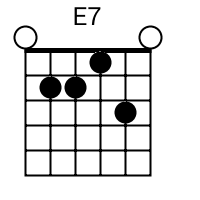
\includegraphics[width = 3cm]{../Akordy/e7.png}
 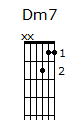
\includegraphics[width = 3cm]{../Akordy/dm7.png}

 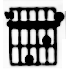
\includegraphics[width = 3cm]{../Akordy/esm7.png}
 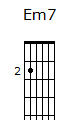
\includegraphics[width = 3cm]{../Akordy/em7.png}



\end{varwidth}

\end{centerjustified}
\setcounter{Slokočet}{0}
\end{song}

\end{document}	